\chapter{Introduction}
\section{Parallel sparse matrix-vector multiplication} \label{sec:par_matvec}
Matrices are one of the most important mathematical objects, as they can be used to represent a wide variety of data in many scientific disciplines: they can encode the structure of a graph, define Markov chains with finitely many states, or possibly represent linear combinations of quantum states or also the behaviour of electronic components. 

In most real-world computations, the systems considered are usually of very large size and involve \textbf{sparse} matrices, because the variables at hand are usually connected to a limited number of others (for example, a very large graph in which each node has just a handful of incident edges); therefore, the matrices involved have the vast majority of entries equal to 0.

More formally, let us consider a matrix of size $m \times n$ with $N$ nonzeros. We say that the matrix is sparse if $ N \ll mn $. Without loss of generality, we assume that each row and column has at least one nonzero (otherwise those rows and columns can easily be removed from the problem).

One of the most fundamental operations performed in these real-world computations is the sparse matrix-vector multiplication, in which we compute

\begin{align}
	u:=Av,
	\label{uAv}
\end{align}

where $A$ denotes our $m \times n$ sparse matrix, $v$ denotes a dense vector of length $n$, and $u$ the resulting vector of length $m$.

The computation of this quantity following the definition of matrix-vector multiplication, i.e. with the sum 

\[ 
	u_i = \sum_{j=0}^{n-1} a_{ij} v_j, \quad \text{for }\; 0 \leq i < m,
\]

requires $\mathcal{O}(n^2) = \mathcal{O}(mn)$ operations; this is not very efficient if we have a sparse matrix: if we perform the multiplications only on the nonzero elements, we obtain an algorithm with running time $\mathcal{O}(N)$, and by definition of sparsity we have that $N \ll mn$.

As mentioned, the systems considered are very large, with sparse matrices with thousands (even millions) of rows and columns and millions of nonzeros; for such big instances, even a running time of $\mathcal{O}(N)$ might be non-negligible, especially since sparse matrix-vector multiplications are usually just a part of a bigger iterative algorithm, and need to be performed several times.

It is a very important goal then to be able to perform such computations in the least amount of time possible: however, as there is a natural tradeoff between power consumption and the speed of the processing units \cite{rabaey1996digital}, it is not feasible to rely only on very fast CPUs, but rather focus on parallelism and employ a large number of them with lower processing speed (and, as a result, with fairly low energy requirements).

To describe an efficient way of performing parallel sparse matrix-vector multiplications, we follow the approach described in \cite{BSP}: before the actual computation takes place, the sparse matrix is distributed among the $p$ processors, creating a \textbf{partitioning} of the set of the nonzeros: $A$ is split into $A_0,\dots,A_{p-1}$ disjoint subsets. Moreover, also the input vector $v$ and the output vector $u$ are distributed among the $p$ processors (note that their distribution might not necessarily, and usually it is not, the same).

Figure \ref{fig:partition} shows a possible partitioning of a $9 \times 9$ matrix with 18 nonzeros. As the the actual values of the nonzeros are not important, we only show the sparsity pattern (a colored cell means that there is a nonzero in that position). The two colors denote, respectively, the two resulting subsets of nonzeros. 

\begin{figure}[h]
	\centering
%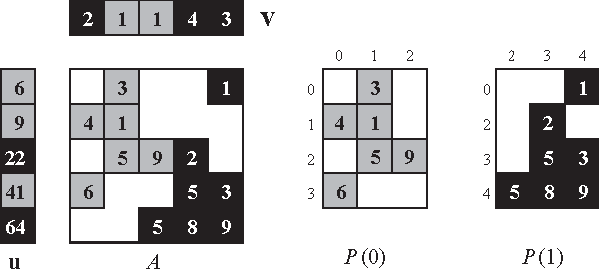
\includegraphics{img/partition}
	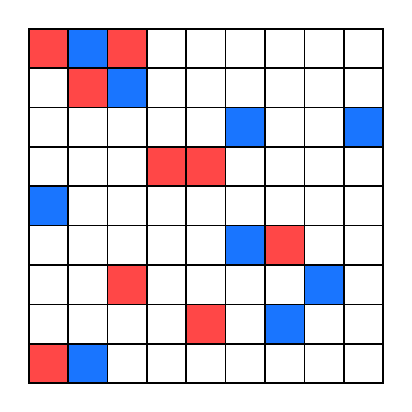
\begin{tikzpicture}[scale=0.5]
		\foreach \x / \y in {1/1,1/3,2/2,4/5,4/4,7/3,8/5,6/7,9/1} { \fill[red!90,opacity=.8] ({\y-1},{-\x+1}) rectangle +(1,-1);}
		\foreach \x / \y in {1/2,2/3,3/6,3/9,6/6,5/1,7/8,8/7,9/2} { \fill[blue!60!cyan,opacity=.9] ({\y-1},{-\x+1}) rectangle +(1,-1);}
		\draw[semithick] (0,-9) grid (9,0);
		\draw[thick] (0,-9) rectangle (9,0);
	\end{tikzpicture}
	\caption{Example of a distribution among two processors of a $9 \times 9$ matrix with 18 nonzeros. Only the sparsity patterns is considered.}
	\label{fig:partition}
\end{figure}

After this distribution, every processor has to compute its local contribution toward the matrix-vector multiplication: to do so, it requires the appropriate vector components which might have been assigned to another processor during the data distribution; if this is the case, communication is required. Once all the required vector components are obtained, the processor starts computing all its local contributions, which are afterwards sent to their appropriate owner, according to the distribution of $u$. The three phases that describe this process for processor $s=0,\dots,p-1$, are summarized in Algorithm \ref{alg:matvec}, from \cite{BSP,mondriaan}.  

\begin{algorithm}[h]
	\begin{algorithmic}
		\Require{$A_s$, the local part of the vector $v$}
		\Ensure{The local part of the vector $u$}
		\State
		\State 	$I_s := \left\{ i | a_{ij} \in A_s \right\}$
		\State 	$J_s := \left\{ j | a_{ij} \in A_s \right\}$
		\State
	\end{algorithmic}
	\begin{enumerate}[(1)]
			\setcounter{enumi}{-1}
		\item 	\begin{algorithmic} \Comment{Fan-out}
				\ForAll{$j \in J_s$}
				\State Get $v_j$ from the processor that owns it. 
				\EndFor
				\State
			\end{algorithmic}
		\item
			\begin{algorithmic} \Comment{Local sparse matrix-vector multiplication}
				\ForAll{$i \in I_s$}
				\State $u_{is} :=0$.
				\ForAll{$j$ such that $a_{ij} \in A_s$}
				\State $u_{is} = u_{is} + a_{ij}v_j$.
				\EndFor
				\EndFor
				\State
			\end{algorithmic}
		\item
			\begin{algorithmic} \Comment{Fan-in}
				\ForAll{$i \in I_s$}
				\State Send $u_{is}$ to the owner of $u_i$.
				\EndFor
				\State
			\end{algorithmic}
	\end{enumerate}
	\label{alg:matvec}
	\caption{Parallel sparse matrix-vector multiplication.}
\end{algorithm}

In reality there is also a fourth phase, in which each processor sums up all the contributions received in phase (2) for all of its owned components of $u$; this is a very small sum with negligible computational cost and for this reason it has been omitted from the algorithm. 

Note that we assume that all of the nonzero values are all represented with the same amount of bits. Doing so, we can focus excusively on the coordinates of the nonzeros, omitting completely their values, as it does not the cost of a parallel sparse matrix-vector multiplication.

Figure \ref{fig:communication} shows an example of the communication involved in supersteps (0) and (2), with the example partitioning shoed in Figure \ref{fig:partition}: the vertical arrows represent the fan out, while the horizontal arrows represent the fan in; the color of an arrow indicates which processor is sending data. 

\begin{figure}[h]
	\centering
	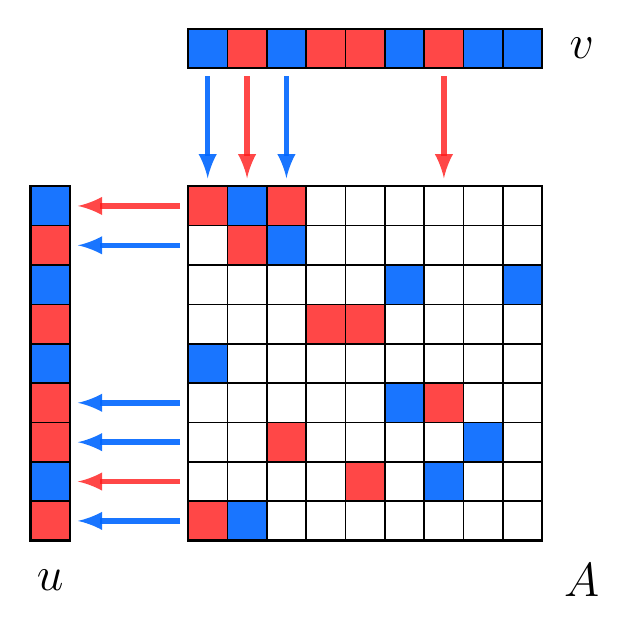
\begin{tikzpicture}[font=\LARGE,scale=0.5]
		\foreach \x / \y in {1/1,1/3,2/2,4/5,4/4,7/3,8/5,6/7,9/1} { \fill[red!90,opacity=.8] ({\y-1},{-\x+1}) rectangle +(1,-1);}
		\foreach \x / \y in {1/2,2/3,3/6,3/9,6/6,5/1,7/8,8/7,9/2} { \fill[blue!60!cyan,opacity=.9] ({\y-1},{-\x+1}) rectangle +(1,-1);}

		\draw[semithick] (0,-9) grid (9,0);
		\draw[thick] (0,-9) rectangle (9,0);

		\foreach \x in {2,4,5,7} { \fill[red!90,opacity=.8] ({\x-1},4) rectangle +(1,-1);}
		\foreach \x in {1,3,6,8,9} { \fill[blue!60!cyan,opacity=.9] ({\x-1},4) rectangle +(1,-1);}

		\foreach \x in {1,3} { \draw[line width=2pt,blue!60!cyan,opacity=.9,->,>=latex] ({\x-0.5},2.8) -- ({\x-0.5},0.2);}
		\foreach \x in {2,7} { \draw[line width=2pt,red!90,opacity=.8,->,>=latex] ({\x-0.5},2.8) -- ({\x-0.5},0.2);}
%	\draw[->,very thick,>=latex] ({7-0.5},1.8) -- ({7-0.5},{-7+0.2});
		\draw[semithick] (0,3) grid (9,4);
		\draw[thick] (0,3) rectangle (9,4);

		\foreach \x in {2,4,6,7,9} { \fill[red!90,opacity=.8] (-4,{-\x+1}) rectangle +(1,-1);}
		\foreach \x in {1,3,5,8} { \fill[blue!60!cyan,opacity=.9] (-4,{-\x+1}) rectangle +(1,-1);}

		\foreach \x in {1,8} { \draw[line width=2pt,red!90,opacity=.8,->,>=latex] (-0.2,{-\x+0.5}) -- (-2.8,{-\x+0.5});}
		\foreach \x in {2,6,7,9} { \draw[line width=2pt,blue!60!cyan,opacity=.9,->,>=latex] (-0.2,{-\x+0.5}) -- (-2.8,{-\x+0.5});}
		\draw[semithick] (-4,-9) grid (-3,0);
		\draw[thick] (-4,-9) rectangle (-3,0);
		\node at (-3.5,-10) {$u$};
		\node at (10,3.5) {$v$};
		\node at (10,-10) {$A$};
	\end{tikzpicture}


%	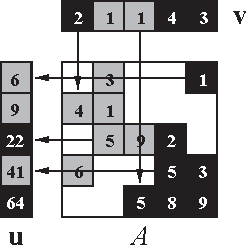
\includegraphics{img/communication}
	\caption{Communication for the sparse parallel matrix-vector multiplication with a matrix partitioned as in Figure \ref{fig:partition}. Vertical arrows represent step (0) while horizontal ones represent step (2). The color of an arrow denotes which processor is sending their data for that row/column.}
	\label{fig:communication}
\end{figure}

As our main interest is to \textbf{minimize} the time spent by the parallel machine computing this sparse matrix-vector multiplication, we need to compute explicitly the cost of Algorithm \ref{alg:matvec}: we can immediately note that such an algorithm, which follows the Bulk Synchronous Parallel model \cite{bsp_paper}, consists of two communication supersteps separated by a computation superstep.

The time spent by a parallel machine in a computation superstep is exactly the time taken by the processor that finishes last: more formally, the time cost of step (1):

\begin{align}
	T_{(1)} = \max_{0 \leq s < p } |A_s|.
	\label{eq:T_comp}
\end{align}

It is easy to understand that, in order to have efficient parallelization, the computation load has to be distributed evenly. Usually, however, it is not possible to achieve a perfect load balance (e.g. when dividing up an odd number of computations among an even number of processors) and we have to reason in terms of an allowed imbalance $\varepsilon$. Consequently, we impose the following hard constraint about the maximum size of the subsets of nonzeros assigned to each processor, according to \cite[eq.~4.27]{BSP}:

\begin{align}
	\max_{0 \leq s <p} |A_s| \leq (1+\varepsilon) \frac{N}{p}.
	\label{eq:balance}
\end{align}

Typical values for the allowed $\varepsilon$ in this constraint are 0.03, i.e. a 3\% imbalance.

It is reasonable, after all, that the problem of finding an efficient way of performing this computation step boils simply down to a hard constraint for the data distribution. This is because we still have to perform all the multiplications of the form $a_{ij} v_j$, no matter our choice. The communication costs, represented by the first and last supersteps in Algorithm \ref{alg:matvec}, are instead the most interesting aspect about maximizing the efficiency of a parallel sparse-matrix vector multiplication algorithm, as there is extreme variability. As a simple example, suppose $p=2$ and consider the matrix represented in Figure \ref{fig:checkered_matrix}. 

\begin{figure}[h]
	\centering
	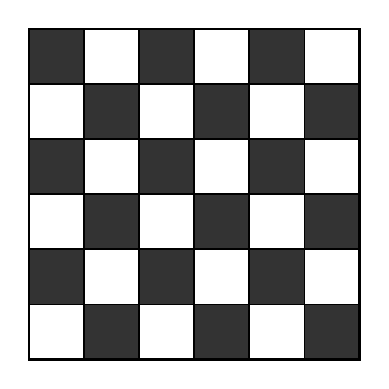
\begin{tikzpicture}[scale=0.7]
		\draw[thick] (0,0) rectangle (6,-6);
		\foreach \row in {0,1, ..., 5} {
			\foreach \column in {0, ..., 2} {
				\fill[opacity=.8] ({2*\column + mod(\row,2)}, -\row) rectangle +(1,-1);
			}
		};
		\draw[semithick] (0,-6) grid (6,0);
	\end{tikzpicture}
	\caption{Example matrix with checkered sparsity pattern. Black boxes represent the nonzeros.} \label{fig:checkered_matrix}
\end{figure}

Two possible partitioning of this matrix into two sets are given in Figure \ref{fig:checkered_partitions}. In Figure \ref{fig:checkered_a} no communication is necessary, whereas in Figure \ref{fig:checkered_b}, all of the rows and columns are split, and therefore the maximum possible communication is required during the sparse matrix vector multiplication algorithm.

\begin{figure}[h]
	\centering
	\subfigure[Rows and columns are not split, therefore there is no need for communication.]{
		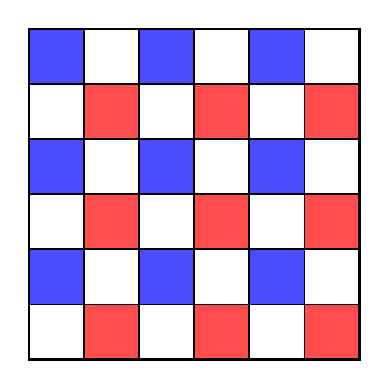
\begin{tikzpicture}[scale=0.7]
			\foreach \row in {0,2,4} {
				\foreach \column in {0, ..., 2} {
					\fill[opacity=.7,blue] ({2*\column + mod(\row,2)}, -\row) rectangle +(1,-1);
				}
			};
			\foreach \row in {1,3,5} {
				\foreach \column in {0, ..., 2} {
					\fill[opacity=.7,red] ({2*\column + mod(\row,2)}, -\row) rectangle +(1,-1);
				}
			};
			\draw[semithick] (0,-6) grid (6,0);
			\draw[thick] (0,0) rectangle (6,-6);
		\end{tikzpicture} \label{fig:checkered_a}
	}\hspace{1cm}
	\subfigure[Every row and column is split and causes communication during fan-in and fan-out.]{
		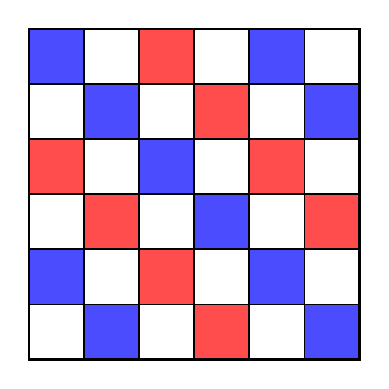
\begin{tikzpicture}[scale=0.7]
			\foreach \index in {0,1, ..., 5} {\fill[opacity=.7,blue] (\index, -\index) rectangle +(1,-1);};
			\foreach \index in {0,1, ..., 3} {\fill[opacity=.7,red] (2+\index, -\index) rectangle +(1,-1);};
			\foreach \index in {0,1, ..., 3} {\fill[opacity=.7,red] (\index, -2-\index) rectangle +(1,-1);};
			\foreach \index in {0,1} {\fill[opacity=.7,blue] (\index, -4-\index) rectangle +(1,-1);};
			\foreach \index in {0,1} {\fill[opacity=.7,blue] (4+\index, -\index) rectangle +(1,-1);};
			\draw[semithick] (0,-6) grid (6,0);
			\draw[thick] (0,0) rectangle (6,-6);
		\end{tikzpicture} \label{fig:checkered_b}
	}
	\caption{Different partitionings of the matrix from Figure \ref{fig:checkered_matrix}. Red and blue squares represent nonzeros assigned to the two different processors.} \label{fig:checkered_partitions}
\end{figure}

Previously, we claimed that the matrix and both the vectors have to be partitioned: in reality it is sufficient to consider only the problem of distributing the nonzeroes, and the partitioning of the vector can be executed according to this: because of the structure of the communication supersteps in Algorithm \ref{alg:matvec}, we have that communication is required if and only if the rows/columns of the matrices are \emph{cut}, i.e. assigned to more than one processor.

If a full column of our matrix $A$ is assigned to the same processor, we can freely assign the corresponding component of $v$ to the same processor, eliminating completely one source of communication (namely, the fan-out for that column). The same reasoning can be done for the rows. This simplification is possible because imposing a hard constraint similar to \eqref{eq:balance} also to the vector distribution is not very helpful, as it only affects the time of linear vector operations outside the matrix-vector multiplication, which are in generally much cheaper \cite[Sec.~3]{mondriaan}. 

We can describe more formally the communications cost, following the notation of \cite[Def.~2.1]{mondriaan}: let $A_0,\dots,A_{p-1}$ be a $p$-way (with $p \geq 1$) partitioning of the sparse matrix $A$ of size $m \times n$. Let $\lambda_i$ denote the number of processors which have a nonzero of row $i$ and let $\mu_j$ be the number of processors that have a nonzero of column $j$; note that, because we assumed that all the rows and columns are nonempty, we have that $\lambda_i, \mu_j \geq 0$.

Then the total time costs for the communication steps in our Algorithm \ref{alg:matvec} are:

\begin{align}
	\begin{aligned}
		T_{(0)} &= \sum_{j=0}^{n-1} (\mu_j -1), \\
		T_{(2)} &= \sum_{i=0}^{m-1} (\lambda_i -1).
	\end{aligned} \label{eq:T_comm}
\end{align}

These costs are quite straightforward: it is reasonable to assume that the owner of the appropriate vector component is one of the processors that have a nonzero in that row/column, and therefore communication is not necessary. Adding these costs together, we define the \textbf{communication volume} $V$ of the considered partitioning as

\begin{align}
	V := V(A_0,\dots,A_{p-1}) = T_{(0)} + T_{(2)} = \sum_{i=0}^{m-1} (\lambda_i -1) + \sum_{j=0}^{n-1} (\mu_j-1).
	\label{eq:volume}
\end{align}

As we can see, the communication volume $V$ depends entirely on the matrix $A$ and the considered partitioning. Therefore, the problem of minimizing the cost of a matrix-vector multiplication is shifted toward finding an efficient way of distributing the sparse matrix among the available processors, such that our balance constraint \eqref{eq:balance} is satisfied. The following sections and chapters and, ultimately, this whole Master Thesis, are therefore dedicated to it.

\section{Hypergraph model}

The problem of distributing the nonzeros of a matrix in order to minimize the communication volume, or, in short, the matrix partitioning problem, can also be viewed from the graph theory point of view. We recall that a (unweighted, undirected) graph $G=(V,E)$ is a set of vertices (or nodes) $V$ and edges $E$ which connect them. 

The graph partitioning problem has been used in the past to model the load balancing in parallel computing: data are represented as vertices, while their connections (the dependencies) are represented with edges. For a more rigorous definition of the graph partitioning problem, we follow the notation given in \cite{hypergraph_model},  performing the simplification in which all the edges have unitary weight. Given the graph $G=(V,E)$ we say that $(V_0,\dots,V_{p-1})$ is a $p$-way partitioning of $G$ if all these subsets are nonempty, mutually disjoint and their union is the whole set of nodes $V$. 

Moreover, we can consider a balance criterion similar to \eqref{eq:balance}:
\begin{align}
	\max_{0\leq s <p}	|V_s| \leq (1+\varepsilon)\frac{|V|}{p},
	\label{eq:balance_hypergraph}
\end{align}

where $\varepsilon$, similarly as before, represents the allowed imbalance.

Now, given a partition $(V_0,\dots,V_{p-1})$ of the graph $G$, we say that the edge $e=(i,j)$ is \emph{cut} if $i \in V_k, j \in V_l$, with $k \neq l$; otherwise, it is said to be \emph{uncut}. Previously, we claimed that communication during the parallel matrix-vector multiplication can be avoided if a row/column is uncut, and here the goal is the same: we want to minimize the \emph{cutsize}, i.e. the number of edges cut.

However, despite all the similarities between the matrix partitioning problem and the graph partitioning one, it has been shown \cite{hypergraph_model}\cite{zoltan_worth-it},  that this cut-edge metric is not an accurate representation of the communication volume. Additional criticism \cite{hendrickson_emperor} comes from the fact that the graph partitioning approach can only handle square symmetric matrices. It was also shown \cite{hendrickson_kolda} that these disadvantages hold for all application of graph partitioning in parallel computing, and not only our problem of matrix partitioning for sparse matrix-vector multiplication. An exact way of modeling the matrix partitioning problem is through the concept of hypergraph partitioning \cite{hypergraph_model}.

A hypergraph is simply a generalization of a graph: we do not consider edges that connect two nodes, but rather \emph{hyperedges} (or \emph{nets}), which are subsets of nodes. Apart from considering only non-empty hyperedges, note that there is no other restriction on their cardinality.

Hypergraphs, and in particular the hypergraph partitioning problem are already well known in literature: they have a natural application in the designing of integrated circuits (VLSI), in finding efficient storage of large databases on disks, and data mining \cite{vlsi}, as well as urban transportation design and study of propositional logic \cite{papa_hypergraph}.

Because of this extensive application basis, translating our matrix partitioning problem to a hypergraph partitioning problem seems quite convenient, as all the methods already developed can be analyzed and employed also in our case.

Figure \ref{fig:hypergraph} shows an example of such a hypergraph. Each colored set represents a different hyperedge; we can see that we can have hyperedges which contain only one node.

\begin{figure}[h]
	\centering
	%\documentclass{article}
%\pagestyle{empty}
%\usepackage{tikz}

\tikzstyle{vertex} = [fill,shape=circle,node distance=80pt]
\tikzstyle{edge} = [fill,opacity=.5,fill opacity=.5,line cap=round, line join=round, line width=50pt]
\tikzstyle{elabel} =  [fill,shape=circle,node distance=35pt]

\pgfdeclarelayer{background}
\pgfsetlayers{background,main}

%\begin{document}
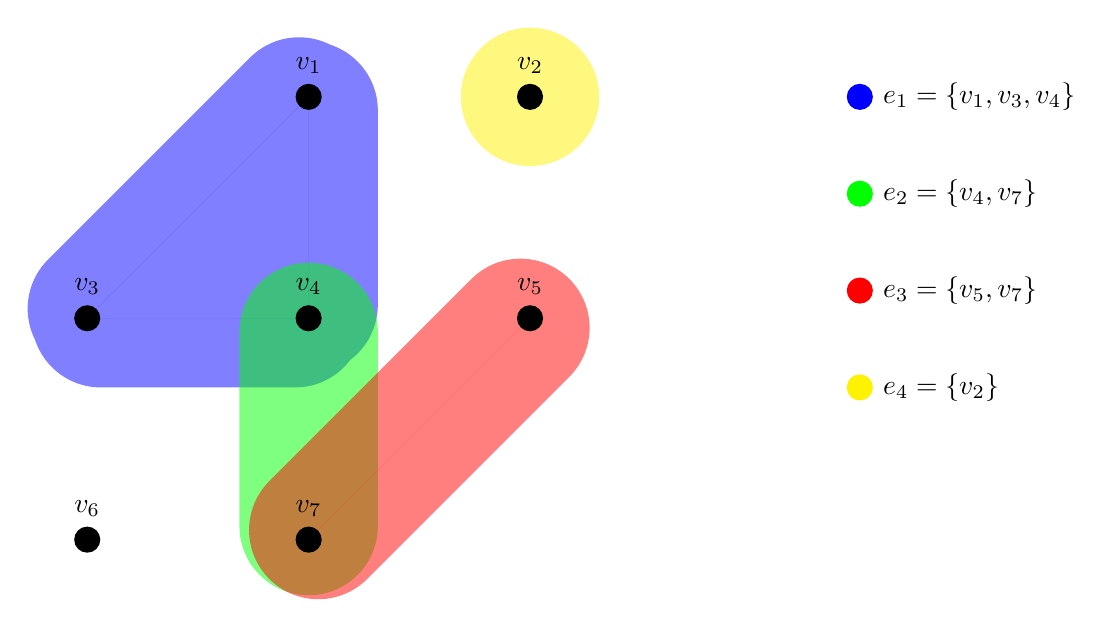
\begin{tikzpicture}
\node[vertex,label=above:\(v_1\)] (v1) {};
\node[vertex,right of=v1,label=above:\(v_2\)] (v2) {};
\node[vertex,below of=v1,label=above:\(v_4\)] (v4) {};
\node[vertex,right of=v4,label=above:\(v_5\)] (v5) {};
\node[vertex,left of=v4,label=above:\(v_3\)] (v3) {};
\node[vertex,below of=v4,label=above:\(v_7\)] (v7) {};
\node[vertex,left of=v7,label=above:\(v_6\)] (v6) {};

\begin{pgfonlayer}{background}
\draw[edge,color=blue] (v1) -- (v3) -- (v4) -- (v1);
\begin{scope}[transparency group,opacity=.5]
\draw[edge,opacity=1,color=green] (v4) -- (v7);
%\fill[edge,opacity=1,color=green] (v3.center) -- (v5.center) -- (v6.center) -- (v3.center);
\end{scope}
\draw[edge,color=red] (v5) -- (v7);
\draw[edge,color=yellow] (v2) -- (v2);
%\draw[edge,color=blue] (v6) -- (v6);
\end{pgfonlayer}

\node[elabel,color=blue,label=right:{$e_1=\{v_1,v_3,v_4\}$}]  (e1) at (7,0) {};
\node[elabel,below of=e1,color=green,label=right:{$e_2=\{v_4,v_7 \}$}]  (e2) {};
\node[elabel,below of=e2,color=red,label=right:{$e_3=\left\{ v_5,v_7 \right\}$}]  (e3) {};
\node[elabel,below of=e3,color=yellow,label=right:{$e_4=\left\{ v_2 \right\}$}]  (e4) {};
\end{tikzpicture}
%\end{document}
 %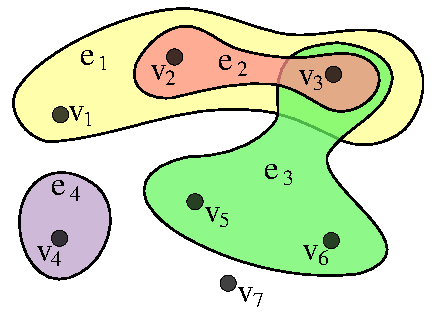
\includegraphics{img/hypergraph}
	\caption{Example of a hypergraph with 7 nodes and 4 hyperedges.}
	\label{fig:hypergraph}
\end{figure}

The definition of hypergraph partitioning problems is identical to the case of a graph, with the difference that now we do not have cut edges, but cut hyperedges: given the hyperedge $e=\{v_1,\dots,v_k\}$, we say that $e$ is cut if there are $i,j$ such that $v_i \in V_r, v_j \in V_s$, with $r \neq s$, i.e. at least two nodes belong to different sets of the partition. As usually, we want to minimize the cut hyperedges.

If, similarly to \eqref{fig:communication}, we define $\lambda_e$ as the number of different sets the vertices in the hyperedge $e$ are assigned to, we have that the total cost of the partition $(V_0,\dots,V_p)$ is:

\begin{align}
	C = C(V_0,\dots,V_{p-1}) = \sum_{e \in E} (\lambda_e -1).
	\label{eq:cost_hypergraph}
\end{align}

We can see how closely these equations resemble the ones given in the previous section: it is clear that the hypergraph partitioning problem closely resembles our original matrix partitioning problem.

Note that the partitioning hypergraph model, along with the simple graph partitioning problem, are known to be NP-hard \cite[Ch.~6]{lengauer}. 

Now, we will describe three possible models for the decomposition of a sparse matrix into a hypergraph, and discuss their advantages and disadvantages.

In the \textbf{column-net} model, our matrix $A$ is represented as a hypergraph for a row-wise decomposition: rows of the matrix are nodes ($V=\{v_1,\dots,v_m\}$, while columns are hyperedges ($E= \{e_1,\dots,e_n\}$). We have that the node $v_i$ belongs to the hyperedge $e_j$ (in short $v_i \in e_j$) if and only if $a_{ij} \neq 0$. With this model, we have that the size of the hyperedge $e_j$ is exactly the number of nonzeros in that column, whereas the node $v_i$ belongs exactly to as many hyperedges as there are nonzeros in that row.

As already said, performing a partitioning on the hypergraph consists of assigning each vertex to one of the sets $V_0,\dots,V_{p-1}$. In this model, this corresponds to assigning a row completely to a processor.However, as vertices are not exactly nonzeros of our matrix, \eqref{eq:balance} and \eqref{eq:balance_hypergraph} are not exactly equivalent; we need to adjust our balance constraint by introducing a weight for each vertex, as in \cite[Def.~4.34]{BSP}. For $v_i \in V$, we define its weight $c_i$ as

\[
	c_i := |\{\;j : \;a_{ij} \neq 0\}|,
\]

which simply is the number of nonzeros in row $i$ of the matrix $A$. Note that, following the same notation as in the previous section, we can see the total number of nonzeros $N$ as $N = \sum_{v_i \in V} c_i$.

Our modified balance constraint is as follows:

\begin{align}
	\max_{0 \leq s <p}	W(V_s) := \max_{0 \leq s <p} \sum_{v_i \in V_s} c_i \leq (1 + \varepsilon) \frac{N}{p}.
	\label{eq:balance_columnet}
\end{align}

The \textbf{row-net} model is very similar to the one just described (as can be guessed from the name): it is exactly the transposed of the colum-net model, in the sense that now rows are hyperedges and columns are vertices of the hypergraph. The reasoning just described applies also to this model, with the little modification that now the weight of a vertex is the number of nonzeros in that column.

We see how the column-net model and row-net model have the advantage of fully assigning a row (or a column) to a processor; this has the advantage of eliminating completely one source of communication in our parallel sparse matrix-vector multiplication algorithm (respectively, the fan-in and fan-out). However, this advantage can easily become a weakness, because now the partitioning is forcedly 1-dimensional, and this is usually too strong of a restriction.

Now, as a last example of possible decomposition of a matrix into a hypergraph, and as a partial address to the drawbacks of the previous two models, we will describe a 2-dimensional approach, the so-called \emph{fine-grain} model \cite{hypergraph_finegrain}. In this model, we have that the $N$ nonzeros are the vertices ($V = \{ v_1,\dots,v_N\}$) and the $m$ rows and $n$ columns are hyperedges ($E = E_r \cup E_c = \{ e_1,\dots,e_m \} \cup \{e_{m+1},\dots,e_{m+n}\}$). With this notation, $E_r$ represents the row hyperedges and $E_c$ represents the column hyperedges. The relationship between the vertices and the hyperedges is fairly obvious: $v_k = a_{ij}$ is in both $e_i$ and $e_{m+j}$.

Now, as the vertices correspond exactly to nonzeros of our matrix, we can use the original equation \eqref{eq:balance_hypergraph} as balance constraint; if we combine this with \eqref{eq:cost_hypergraph}, which describes the cost of a hypergraph partition, we can clearly see how this is identical to our original matrix partitioning problem, described by \eqref{eq:balance} and \eqref{eq:volume}.

On a higher level, one of the benefits of this decomposition model is easy to understand: we have a lot of freedom and we can assign individually each nonzero to a different partition. Similarly as before, however, this advantage can easily become a drawback because now the size of the hypergraph is consistently larger, with $N$ vertices compared to $m$ and $n$ of the previous two models. Thus, computations on the fine-grain model take substantially more time than row-net or column-net models and therefore there is a restriction on the size of the problem that can be efficiently solved.

\section{Earlier work}

Among the models used to translate matrix partitioning into hypergraph partitioning, we already mentioned row-net and column-net \cite{hypergraph_model}, proposed in 1999, and a more recent fine-grained approach \cite{hypergraph_finegrain}, proposed in 2001. New models are relatively rare, and recently Pelt and Bisseling proposed the interesting \textbf{medium-grain} model .  \cite{mediumgrain}.  As this model is at the very base of our work, a more detailed explanation will be given in Section \ref{sec:mediumgrain}.

In addition to these models, there has been some research effort towards the creation of more complicated methods, which often comprise several stages and combine different models.

For example, Uçar and Aykanat \cite{hypergraph_revisiting} first employ an elementary 1-dimensional hypergraph model, and then they transform it in several ways to different hypergraph models suitable for both symmetric and unsymmetric matrix partitionings; it is important to note that these models also include the input and output vectors, and therefore a few extra vertices are added to the hypergraph.

A different 2-dimensional approach is given by the \emph{coarse-grain} method \cite{hypergraph_coarsegrain}: first the column-net hypergraph model is used, obtaining a row partitioning of the matrix in $p$ parts, then a multi-constraint column partitioning in $q$ parts is performed, yielding a final 2-D cartesian partitioning in $p \times q$ parts. 

Moreover, Vastenhouw and Bisseling proposed a 2-dimensional recursive method for data distribution \cite{mondriaan}; this greedy method splits recursively a rectangular matrix into 2 parts.
At each step of the recursion, there is the choice on the direction to be taken in the next step: two different strategies are proposed, alternating splitting directions or simply trying to split both vertically and horizontally and taking greedily the best of the two.

Besides these general purpose models and methods, it is also possible to take into account the structure of the matrix to be partitioned: the hypergraph-based approach was indeed initially devised for structurally symmetric matrices \cite{hypergraph_model}. Moreover, Hu, Maguire and Blake present in \cite{hu2000} an algorithm for nonsymmetric matrices that performs row and column permutations, getting a bordered block diagonal form and then trying to assign matrix rows such that the number of cut columns is minimized.

In general, as there is such a wide variety of different methods and model, it might be difficult to choose the best one, given a matrix to partition. {\c{C}}ataly{\"u}rek, Aykanat, and U{\c{c}}ar propose a partitioning recipe \cite{catalyurek_recipe} that chooses a partitioning method according to some matrix characteristics.

Regarding the actual implementations of the just discussed models, methods and algorithms, there are a few existing software partitioners available. Among the sequential ones we have PaToH (a multilevel Partitioning Tool for Hypergraphs) \cite{patoh}, hMetis \cite{hmetis} (specifically targeted at partitioning hypergraphs for VLSI design), Mondriaan \cite{mondriaan} (among the ones here described, this is the one more specifically designed to solve the matrix partitioning problem), MONET (Matrix Ordering for minimal NET-cut)\cite{hu2000}. Zoltan-PHG (Parallel Hypergraph Partitioner) \cite{parallel_hypergraph} performs instead matrix partitioning in parallel; the relative scarcity of parallel software partitioners is to be explained by the fact that this field is relatively new, and therefore most of the research efforts have been directed toward a sequential approach.

The partitioners just mentioned produce very different results, with respect to both solution quality and execution time, despite having at the core the same method for finding good initial solutions. The method employed is the well-known Kernighan-Lin \cite{kernighan_lin} method, with the optimizations of Fiduccia-Mattheyses \cite{fiduccia}. This local search heuristic was originally designed for bipartitioning graphs and, given a partitioning that obeys the balance constraint \eqref{eq:balance}, it applies a series of small changes to improve the quality of the solution.

To solve large instances, all these partitioners use a multi-level method: the large problem is progressively coarsened until a smaller instance is obtained, then the problem is solved on this small instance and the solution is gradually uncoarsened, with a refinement at each step to improve the solution quality.

Finally, these existing software partitioners are all based on \emph{recursive bisection}: instead of partitioning the hypergraph directly into the desired number of parts, they execute a sequence of bisections of the partitions. This is a good semplification in the sense that it just suffices to find very good algorithms for bipartitioning, and also because splitting a hypergraph in just two parts is much easier; there is however one major flaw with this approach: using this recursive bisection  we might not be able to reach the same quality of a solution with direct splitting into the desired number of parts.

\section{Medium-grain model} \label{sec:mediumgrain}

All of the possible ways of translating the matrix partitioning problem into a hypergraph partitioning problem have different advantages and drawbacks: the 1-dimensional ones, row-net and colum-net, eliminate completely one source of communication but are somewhat too restrictive; fine-grain, on the contrary, does not provide any kind of limitation on the choices for the partitioning, but the resulting hypergraph is very often too big to manage.

A new model has recently been proposed by Pelt and Bisseling \cite{mediumgrain}, which can be described as a sort of middle ground between the 1-dimensional models and fine-grain model. The resulting partitioning is 2-dimensional by design (thus avoiding the limitations of the row-net and column-net models), but it still imposes that clusters of nonzeros from the same rows and columns are assigned to the same processor, thus reducing the size of the final hypergraph, avoiding the main disadvantage of the fine-grain model.

The key of the medium-grain model lies into the splitting of our original matrix $A$ in two parts, $A_r$ and $A_c$, such that $A_r + A_c = A$. Then, we proceed to construct the auxiliary block-matrix $B$, of size $(m+n) \times (m+n)$, defined as

\begin{align}
	B:=	\begin{bmatrix}
		I_n & A_r^T \\
		A_c & I_m
	\end{bmatrix},
	\label{eq:Bmatrix}
\end{align}

where $I_n$ and $I_m$ denote, respectively, the identity matrices of size $n$ and $m$. The final hypergraph is finally obtained by applying the row-net model to this matrix $B$. 

Figure \ref{fig:mediumgrain-1} illustrates this process for a $3 \times 6$ rectangular matrix $A$.

\begin{figure}[h]
	\centering
%	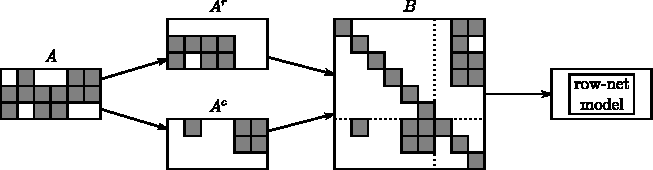
\includegraphics{img/mg-1}
	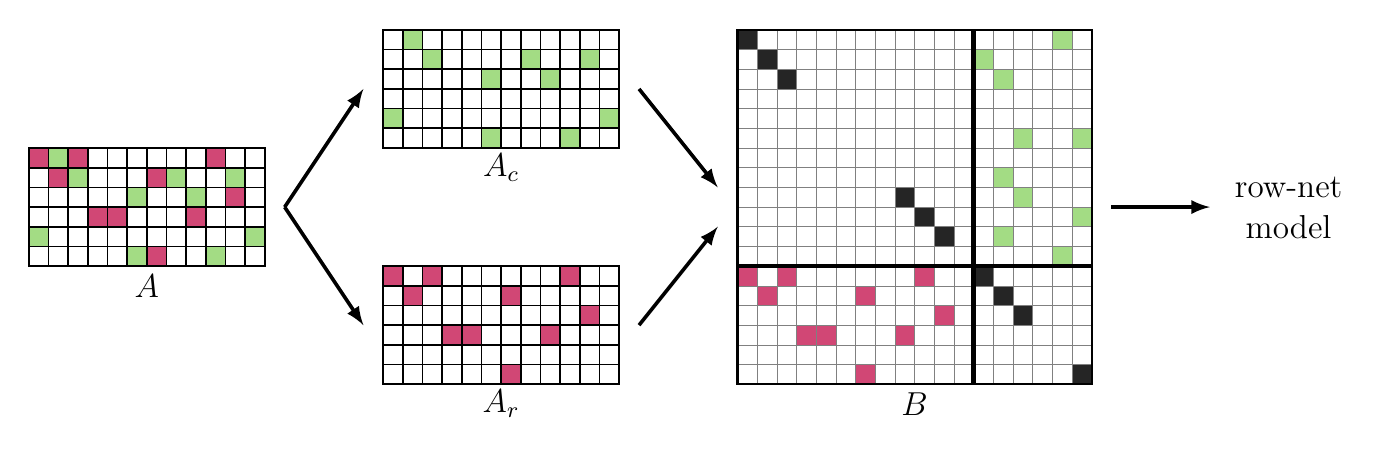
\begin{tikzpicture}[scale=0.25,font=\large]
	\foreach \x / \y in {1/1,1/3,2/2,4/5,4/4,3/11,4/9,6/7,1/10,2/7} { \fill[purple!90,opacity=.8] ({\y-1},{-\x+1}) rectangle +(1,-1);}
	\foreach \x / \y in {1/2,2/3,3/6,3/9,6/6,5/1,5/12,6/10,2/11,2/8} { \fill[yellow!60!cyan,opacity=.9] ({\y-1},{-\x+1}) rectangle +(1,-1);}
	\draw[semithick] (0,-6) grid (12,0);
	\draw[thick] (0,-6) rectangle (12,0);
	\node at (6,-7) {$A$};

	\foreach \x / \y in {1/1,1/3,2/2,4/5,4/4,3/11,4/9,6/7,1/10,2/7}{ \fill[purple!90,opacity=.8] ({18+\y-1},{-6-\x+1}) rectangle +(1,-1);}
	\node at (24,-13) {$A_r$};
	\draw[semithick] (18,{-6-6}) grid ({18+12},-6);
	\draw[thick] (18,{-6-6}) rectangle ({18+12},-6);

	\foreach \x / \y in  {1/2,2/3,3/6,3/9,6/6,5/1,5/12,6/10,2/11,2/8} { \fill[yellow!60!cyan,opacity=.9] ({18+\y-1},{6-\x+1}) rectangle +(1,-1);}
	\node at (24,-1) {$A_c$};
	\draw[semithick] (18,{-6+6}) grid ({18+12},6);
	\draw[thick] (18,{-6+6}) rectangle ({18+12},6);


	\foreach \x / \y in {1/1,1/3,2/2,4/5,4/4,3/11,4/9,6/7,1/10,2/7}{ \fill[purple!90,opacity=.8] ({36+\y-1},{-6-\x+1}) rectangle +(1,-1);}
	\foreach \x / \y in  {1/2,2/3,3/6,3/9,6/6,5/1,5/12,6/10,2/11,2/8} { \fill[yellow!60!cyan,opacity=.9] ({48+\x-1},{6-\y+1}) rectangle +(1,-1);}


	\foreach \x in {1,2,3,9,10,11} { \fill[gray!10!black,opacity=.9] ({36+\x-1},{6-\x+1}) rectangle +(1,-1);}
	\foreach \x in {1,2,3,6} { \fill[gray!10!black,opacity=.9] ({48+\x-1},{-6-\x+1}) rectangle +(1,-1);}

	\draw[very thin,help lines] (36,-12) grid (54,6);
	\draw[thick] (36,-12) rectangle (54,6);
	\draw[ultra thick] (48,-12) -- (48,6);
	\draw[ultra thick] (36,-6) -- (54,-6);

	\node at (45,-13) {$B$};

	\draw[line width=1.3pt,>=latex,->] (13,-3) -- (17,-9);
	\draw[line width=1.3pt,>=latex,->] (13,-3) -- (17,3);
	\draw[line width=1.3pt,>=latex,->] (31,-9) -- (35,-4);
	\draw[line width=1.3pt,>=latex,->] (31,3) -- (35,-2);
	
	\draw[line width=1.3pt,>=latex,->] (55,-3) -- (60,-3);
	\node at (64,-2) {row-net};
	\node at (64,-4) {model};
\end{tikzpicture}
\caption{Example of the construction of the matrix $B$ from a $6 \times 12$ matrix $A$, for which the sets $A_r$ and $A_c$ were previously established and colored differently. In the resulting matrix, the dummy nonzeros are depicted in black.}
	\label{fig:mediumgrain-1}
\end{figure}

After we apply the row-net model and obtain a partitioning of the hypergraph, it is immediate to retrieve a partitioning of our matrix $A$, as depicted in Figure \ref{fig:mediumgrain-2}. 

\begin{figure}[h]
	\centering
%	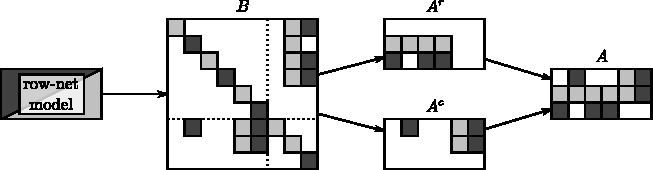
\includegraphics{img/mg-2}
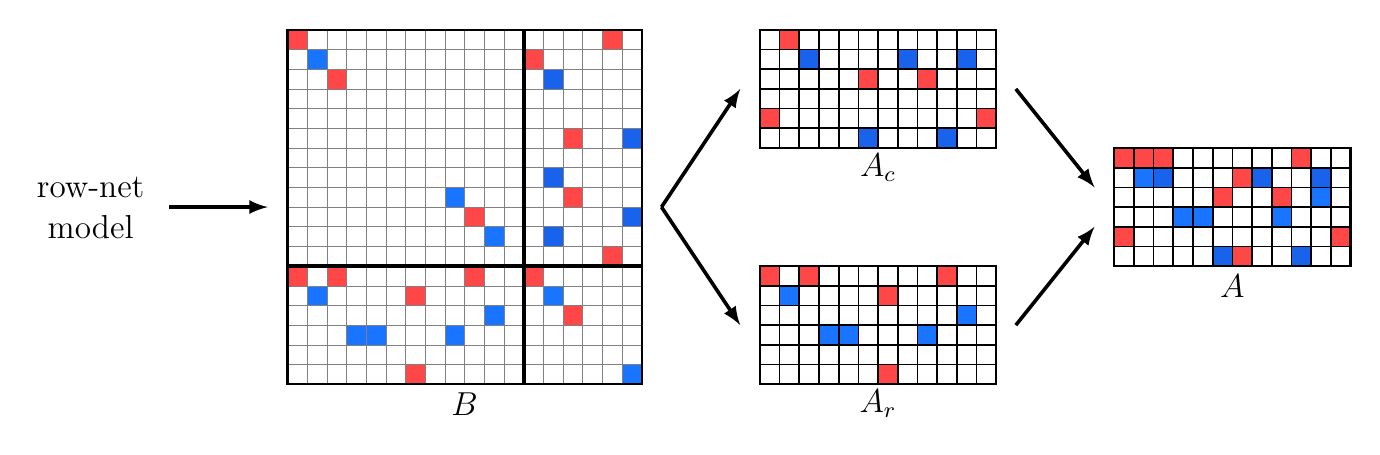
\begin{tikzpicture}[scale=0.25,font=\large]

	\tikzstyle{myred}=[red!90,opacity=.8]
	\tikzstyle{myblue}=[blue!60!cyan,opacity=.9]
	\tikzstyle{myarrow}=[line width=1.3pt,>=latex,->]

	\foreach \x / \y in {1/1,1/3,6/7,1/10,2/7}{ \fill[myred] ({42+\y-1},{-\x+1}) rectangle +(1,-1);}
	\foreach \x / \y in {2/2,4/5,4/4,4/9,3/11}{ \fill[myblue] ({42+\y-1},{-\x+1}) rectangle +(1,-1);}
	\foreach \x / \y in {1/2,2/3,3/6,3/9,6/6,5/1,5/12,6/10,2/11,2/8} { \fill[myred] ({42+\y-1},{-\x+1}) rectangle +(1,-1);}
	\foreach \x / \y in   {2/3,6/6,6/10,2/11,2/8} { \fill[myblue] ({42+\y-1},{-\x+1}) rectangle +(1,-1);}
	\draw[semithick] (42,-6) grid +(12,6);
	\draw[thick] (42,-6) rectangle +(12,6);

	\node at (48,-7) {$A$};

	\foreach \x / \y in {1/1,1/3,6/7,1/10,2/7}{ \fill[myred] ({24+\y-1},{-6-\x+1}) rectangle +(1,-1);}
	\foreach \x / \y in {2/2,4/5,4/4,4/9,3/11}{ \fill[myblue] ({24+\y-1},{-6-\x+1}) rectangle +(1,-1);}

	\node at (30,-13) {$A_r$};
	\draw[semithick] (24,{-6-6}) grid +(12,6);
	\draw[thick] (24,{-6-6}) rectangle +(12,6);

	\foreach \x / \y in {1/2,2/3,3/6,3/9,6/6,5/1,5/12,6/10,2/11,2/8} { \fill[myred] ({24+\y-1},{6-\x+1}) rectangle +(1,-1);}
	\foreach \x / \y in   {2/3,6/6,6/10,2/11,2/8} { \fill[myblue] ({24+\y-1},{6-\x+1}) rectangle +(1,-1);}
	\node at (30,-1) {$A_c$};
	\draw[semithick] (24,{-6+6}) grid +(12,6);
	\draw[thick] (24,{-6+6}) rectangle +(12,6);

	\foreach \x / \y in {1/1,1/3,6/7,1/10,2/7}{ \fill[myred] ({0+\y-1},{-6-\x+1}) rectangle +(1,-1);}
	\foreach \x / \y in {2/2,4/5,4/4,4/9,3/11}{ \fill[myblue] ({0+\y-1},{-6-\x+1}) rectangle +(1,-1);}

	\foreach \x in {1,3,10} { \fill[myred] ({0+\x-1},{6-\x+1}) rectangle +(1,-1);}
	\foreach \x in {2,9,11} { \fill[myblue] ({0+\x-1},{6-\x+1}) rectangle +(1,-1);}


	\foreach \x / \y in  {1/2,2/3,3/6,3/9,6/6,5/1,5/12,6/10,2/11,2/8} { \fill[myred] ({12+\x-1},{6-\y+1}) rectangle +(1,-1);}
	\foreach \x / \y in  {2/3,6/6,6/10,2/11,2/8} { \fill[myblue] ({12+\x-1},{6-\y+1}) rectangle +(1,-1);}


	\foreach \x in {1,3} { \fill[myred] ({12+\x-1},{-6-\x+1}) rectangle +(1,-1);}
	\foreach \x in {2,6} { \fill[myblue] ({12+\x-1},{-6-\x+1}) rectangle +(1,-1);}

	\draw[very thin,help lines] (0,-12) grid +(18,18);
	\draw[thick] (0,-12) rectangle +(18,18);
	\draw[ultra thick] (12,-12) -- +(0,18);
	\draw[ultra thick] (0,-6) -- +(18,0);

	\node at (9,-13) {$B$};
%
	\draw[myarrow] (19,-3) -- +(4,6);
	\draw[myarrow] (19,-3) -- +(4,-6);
	\draw[myarrow] (37,-9) -- +(4,5);
	\draw[myarrow] (37,3) -- +(4,-5);
%	
	\draw[myarrow] (-6,-3) -- (-1,-3);
	\node at (-10,-2) {row-net};
	\node at (-10,-4) {model};
\end{tikzpicture}

	\caption{Process of obtaining a matrix partitioning starting from a partitioning of the hypergraph following the medium-grain model. In this case $p=2$.}
	\label{fig:mediumgrain-2}
\end{figure}

The usefulness of $A_c$ and $A_r$ is clear if we consider that we use the row-net model. The first is left as-is, while the second is transposed; then, when partitioning 1-dimensionally such that the columns are kept together, we see that we are effectively keeping together elements within the same columns of $A_c$ and $A_r^T$. The resulting partitioning is fully 2-dimensional, because we have clusters of nonzeros: rows for $A_r$ and columns for $A_c$ (hence the subscripts).

The diagonal elements of $B$ are used only to compute the communication volume. Let us consider the $k$th column of $A$; the corresponding nonzeros can be found in the $k$th column of $A_c$  and in the $k$th row of $A_r^T$. If both these parts are nonempty, i.e. the $k$th column of $A$ was not fully assigned to either $A_r$ or $A_c$, we need to be careful when we compute the communication volume of a given partitioning: if these parts are to different processors, communication is needed in Algorithm \ref{alg:matvec}.

Therefore the diagonal nonzero $B_{k,k}$, assigned by the row-net model to the same processor as the $k$th column of $A_c$, that belongs to same row of $B$ as the $k$th row of $A_r$, has the purpose of ensuring a correct computation of the communication volume \cite[Th.~3.1]{mediumgrain}. Note that, implementation-wise, there is no need to have the complete diagonal of $B$: we put a nonzero if and only if the corresponding row of $A_r^T$ and column of $A_c$ are both nonempty.

Experimental results, performed with both the Mondriaan and PaToH packages seems to confirm that this model has indeed some advantages compared to the column-net, row-net and fine-grain models, both regarding partitioning time and solution quality.

Because of these good results, it is our goal to investigate further the properties of this model, following two possible directions.

First of all, as the outcome of the medium-grain model depends remarkably on the initial split of $A$ into $A_r$ and $A_c$, it is interesting to investigate the quality of the algorithm originally proposed in \cite{mondriaan} to achieve this initial partitioning; secondly, we will try to develop a fully iterative method that employs the medium-grain model, where a full multi-level partitioning is performed at each iteration and computation time is traded for solution quality.

Both these research directions share a very important part: we just need to develop efficient methods to compute from the given matrix $A$ the matrices $A_r$ or $A_c$ required for the medium grain model, either from scratch or starting from an already existing partitioning (later in the work we will talk, respectively, about \emph{partition-oblivious} and \emph{partition-aware} algorithms). 

To this extent, Chapters \ref{chap:methods} and \ref{chap:independent_set} describe several of these different methods, whereas in Chapter \ref{chap:experimental_results} we discuss their implementation and the experimental results for the two mentioned research directions.
